% Options for packages loaded elsewhere
% Options for packages loaded elsewhere
\PassOptionsToPackage{unicode}{hyperref}
\PassOptionsToPackage{hyphens}{url}
%
\documentclass[
  ignorenonframetext,
  aspectratio=169,
  spanish,
]{beamer}
\newif\ifbibliography
\usepackage{pgfpages}
\setbeamertemplate{caption}[numbered]
\setbeamertemplate{caption label separator}{: }
\setbeamercolor{caption name}{fg=normal text.fg}
\beamertemplatenavigationsymbolshorizontal
% remove section numbering
\setbeamertemplate{part page}{
  \centering
  \begin{beamercolorbox}[sep=16pt,center]{part title}
    \usebeamerfont{part title}\insertpart\par
  \end{beamercolorbox}
}
\setbeamertemplate{section page}{
  \centering
  \begin{beamercolorbox}[sep=12pt,center]{section title}
    \usebeamerfont{section title}\insertsection\par
  \end{beamercolorbox}
}
\setbeamertemplate{subsection page}{
  \centering
  \begin{beamercolorbox}[sep=8pt,center]{subsection title}
    \usebeamerfont{subsection title}\insertsubsection\par
  \end{beamercolorbox}
}
% Prevent slide breaks in the middle of a paragraph
\widowpenalties 1 10000
\raggedbottom
\AtBeginPart{
  \frame{\partpage}
}
\AtBeginSection{
  \ifbibliography
  \else
    \frame{\sectionpage}
  \fi
}
\AtBeginSubsection{
  \frame{\subsectionpage}
}
\usepackage{iftex}
\ifPDFTeX
  \usepackage[T1]{fontenc}
  \usepackage[utf8]{inputenc}
  \usepackage{textcomp} % provide euro and other symbols
\else % if luatex or xetex
  \usepackage{unicode-math} % this also loads fontspec
  \defaultfontfeatures{Scale=MatchLowercase}
  \defaultfontfeatures[\rmfamily]{Ligatures=TeX,Scale=1}
\fi
\usepackage{lmodern}

\usetheme[]{default}
\usefonttheme[]{default}
\ifPDFTeX\else
  % xetex/luatex font selection
\fi
% Use upquote if available, for straight quotes in verbatim environments
\IfFileExists{upquote.sty}{\usepackage{upquote}}{}
\IfFileExists{microtype.sty}{% use microtype if available
  \usepackage[]{microtype}
  \UseMicrotypeSet[protrusion]{basicmath} % disable protrusion for tt fonts
}{}
\makeatletter
\@ifundefined{KOMAClassName}{% if non-KOMA class
  \IfFileExists{parskip.sty}{%
    \usepackage{parskip}
  }{% else
    \setlength{\parindent}{0pt}
    \setlength{\parskip}{6pt plus 2pt minus 1pt}}
}{% if KOMA class
  \KOMAoptions{parskip=half}}
\makeatother

\usepackage{color}
\usepackage{fancyvrb}
\newcommand{\VerbBar}{|}
\newcommand{\VERB}{\Verb[commandchars=\\\{\}]}
\DefineVerbatimEnvironment{Highlighting}{Verbatim}{commandchars=\\\{\}}
% Add ',fontsize=\small' for more characters per line
\usepackage{framed}
\definecolor{shadecolor}{RGB}{241,243,245}
\newenvironment{Shaded}{\begin{snugshade}}{\end{snugshade}}
\newcommand{\AlertTok}[1]{\textcolor[rgb]{0.68,0.00,0.00}{#1}}
\newcommand{\AnnotationTok}[1]{\textcolor[rgb]{0.37,0.37,0.37}{#1}}
\newcommand{\AttributeTok}[1]{\textcolor[rgb]{0.40,0.45,0.13}{#1}}
\newcommand{\BaseNTok}[1]{\textcolor[rgb]{0.68,0.00,0.00}{#1}}
\newcommand{\BuiltInTok}[1]{\textcolor[rgb]{0.00,0.23,0.31}{#1}}
\newcommand{\CharTok}[1]{\textcolor[rgb]{0.13,0.47,0.30}{#1}}
\newcommand{\CommentTok}[1]{\textcolor[rgb]{0.37,0.37,0.37}{#1}}
\newcommand{\CommentVarTok}[1]{\textcolor[rgb]{0.37,0.37,0.37}{\textit{#1}}}
\newcommand{\ConstantTok}[1]{\textcolor[rgb]{0.56,0.35,0.01}{#1}}
\newcommand{\ControlFlowTok}[1]{\textcolor[rgb]{0.00,0.23,0.31}{\textbf{#1}}}
\newcommand{\DataTypeTok}[1]{\textcolor[rgb]{0.68,0.00,0.00}{#1}}
\newcommand{\DecValTok}[1]{\textcolor[rgb]{0.68,0.00,0.00}{#1}}
\newcommand{\DocumentationTok}[1]{\textcolor[rgb]{0.37,0.37,0.37}{\textit{#1}}}
\newcommand{\ErrorTok}[1]{\textcolor[rgb]{0.68,0.00,0.00}{#1}}
\newcommand{\ExtensionTok}[1]{\textcolor[rgb]{0.00,0.23,0.31}{#1}}
\newcommand{\FloatTok}[1]{\textcolor[rgb]{0.68,0.00,0.00}{#1}}
\newcommand{\FunctionTok}[1]{\textcolor[rgb]{0.28,0.35,0.67}{#1}}
\newcommand{\ImportTok}[1]{\textcolor[rgb]{0.00,0.46,0.62}{#1}}
\newcommand{\InformationTok}[1]{\textcolor[rgb]{0.37,0.37,0.37}{#1}}
\newcommand{\KeywordTok}[1]{\textcolor[rgb]{0.00,0.23,0.31}{\textbf{#1}}}
\newcommand{\NormalTok}[1]{\textcolor[rgb]{0.00,0.23,0.31}{#1}}
\newcommand{\OperatorTok}[1]{\textcolor[rgb]{0.37,0.37,0.37}{#1}}
\newcommand{\OtherTok}[1]{\textcolor[rgb]{0.00,0.23,0.31}{#1}}
\newcommand{\PreprocessorTok}[1]{\textcolor[rgb]{0.68,0.00,0.00}{#1}}
\newcommand{\RegionMarkerTok}[1]{\textcolor[rgb]{0.00,0.23,0.31}{#1}}
\newcommand{\SpecialCharTok}[1]{\textcolor[rgb]{0.37,0.37,0.37}{#1}}
\newcommand{\SpecialStringTok}[1]{\textcolor[rgb]{0.13,0.47,0.30}{#1}}
\newcommand{\StringTok}[1]{\textcolor[rgb]{0.13,0.47,0.30}{#1}}
\newcommand{\VariableTok}[1]{\textcolor[rgb]{0.07,0.07,0.07}{#1}}
\newcommand{\VerbatimStringTok}[1]{\textcolor[rgb]{0.13,0.47,0.30}{#1}}
\newcommand{\WarningTok}[1]{\textcolor[rgb]{0.37,0.37,0.37}{\textit{#1}}}

\usepackage{longtable,booktabs,array}
\usepackage{calc} % for calculating minipage widths
\usepackage{caption}
% Make caption package work with longtable
\makeatletter
\def\fnum@table{\tablename~\thetable}
\makeatother
\usepackage{graphicx}
\makeatletter
\newsavebox\pandoc@box
\newcommand*\pandocbounded[1]{% scales image to fit in text height/width
  \sbox\pandoc@box{#1}%
  \Gscale@div\@tempa{\textheight}{\dimexpr\ht\pandoc@box+\dp\pandoc@box\relax}%
  \Gscale@div\@tempb{\linewidth}{\wd\pandoc@box}%
  \ifdim\@tempb\p@<\@tempa\p@\let\@tempa\@tempb\fi% select the smaller of both
  \ifdim\@tempa\p@<\p@\scalebox{\@tempa}{\usebox\pandoc@box}%
  \else\usebox{\pandoc@box}%
  \fi%
}
% Set default figure placement to htbp
\def\fps@figure{htbp}
\makeatother



\ifLuaTeX
\usepackage[bidi=basic]{babel}
\else
\usepackage[bidi=default]{babel}
\fi
% get rid of language-specific shorthands (see #6817):
\let\LanguageShortHands\languageshorthands
\def\languageshorthands#1{}


\setlength{\emergencystretch}{3em} % prevent overfull lines

\providecommand{\tightlist}{%
  \setlength{\itemsep}{0pt}\setlength{\parskip}{0pt}}



 


\setbeamertemplate{headline}{} % Elimina la cabecera del tema Madrid
\setbeamertemplate{section in head/foot}{} % Limpia la numeración de secciones
\renewcommand{\contentsname}{Índice}
\renewcommand{\refname}{Referencias}
\renewcommand{\figurename}{Figura}
\renewcommand{\tablename}{Tabla}
\logo{%
  \begin{tabular}{c}
    
\includegraphics[height=1.2cm]{EscudoU.png}
  \end{tabular}%
}
% --- CONFIGURACIÓN DE COLORES INSTITUCIONALES ---
\definecolor{UnicorGreen}{HTML}{024426}
\definecolor{UnicorText}{HTML}{F9F9F9}
\definecolor{UnicorWhite}{HTML}{FFFFFF}
\definecolor{UnicorGold}{HTML}{D1B061}

% Aplicación al fondo y texto general
\setbeamercolor{background canvas}{bg=UnicorGreen}
\setbeamercolor{normal text}{fg=UnicorText}

% Aplicación a títulos y cabeceras
%\setbeamercolor{title}{fg=UnicorWhite}
\setbeamercolor{frametitle}{fg=UnicorWhite}
\setbeamercolor{framesubtitle}{fg=UnicorWhite}

% Aplicación a viñetas y estructura
\setbeamercolor{structure}{fg=UnicorWhite}
\setbeamercolor{itemize item}{fg=UnicorWhite}
\setbeamercolor{itemize subitem}{fg=UnicorWhite}
\setbeamercolor{enumerate item}{fg=UnicorWhite}

% Forzar a LaTeX a repintar el texto general al iniciar el documento
\AtBeginDocument{\usebeamercolor[fg]{normal text}}

% Aplicación a hipervínculos
\hypersetup{colorlinks=true, urlcolor=UnicorGold, linkcolor=UnicorWhite}

% --- ACTIVAR ESTILO DE BLOQUES Y SOMBRAS (ESTILO MADRID) ---
\useinnertheme[shadow=true]{rounded}

% --- COLORES DEL RECUADRO DEL TÍTULO PRINCIPAL ---
% Fondo dorado con texto verde
\setbeamercolor{title}{bg=UnicorGold, fg=UnicorGreen}
\setbeamercolor{frametitle}{fg=UnicorWhite} % Mantiene el título de las diapositivas normal
\setbeamercolor{framesubtitle}{fg=UnicorWhite}

% --- COLORES PARA TEOREMAS, DEFINICIONES Y BLOQUES ---
% Título del bloque (Fondo dorado, texto verde)
\setbeamercolor{block title}{bg=UnicorGold, fg=UnicorGreen}
% Cuerpo del bloque (Fondo blanco, texto verde)
\setbeamercolor{block body}{bg=UnicorWhite, fg=UnicorGreen}

\AtBeginDocument{
  \author{%
    \begin{tabular}{c}
      Mario A. Morales Rivera \\
      \footnotesize \texttt{mamorales@correo.unicordoba.edu.co} \\
      \footnotesize Universidad de Córdoba
    \end{tabular}
  }
  \institute{}
}
% --- LIMPIAR DIAPOSITIVAS DE SECCIÓN (ELIMINAR "SECTION X") ---
\setbeamertemplate{section page}{
  \begin{center}
    \begin{beamercolorbox}[sep=12pt,center,rounded=true,shadow=true]{title}
      \usebeamerfont{title}\insertsection\par
    \end{beamercolorbox}
  \end{center}
}
\makeatletter
\@ifpackageloaded{caption}{}{\usepackage{caption}}
\AtBeginDocument{%
\ifdefined\contentsname
  \renewcommand*\contentsname{Tabla de contenidos}
\else
  \newcommand\contentsname{Tabla de contenidos}
\fi
\ifdefined\listfigurename
  \renewcommand*\listfigurename{Listado de Figuras}
\else
  \newcommand\listfigurename{Listado de Figuras}
\fi
\ifdefined\listtablename
  \renewcommand*\listtablename{Listado de Tablas}
\else
  \newcommand\listtablename{Listado de Tablas}
\fi
\ifdefined\figurename
  \renewcommand*\figurename{Figura}
\else
  \newcommand\figurename{Figura}
\fi
\ifdefined\tablename
  \renewcommand*\tablename{Tabla}
\else
  \newcommand\tablename{Tabla}
\fi
}
\@ifpackageloaded{float}{}{\usepackage{float}}
\floatstyle{ruled}
\@ifundefined{c@chapter}{\newfloat{codelisting}{h}{lop}}{\newfloat{codelisting}{h}{lop}[chapter]}
\floatname{codelisting}{Listado}
\newcommand*\listoflistings{\listof{codelisting}{Listado de Listados}}
\makeatother
\makeatletter
\makeatother
\makeatletter
\@ifpackageloaded{caption}{}{\usepackage{caption}}
\@ifpackageloaded{subcaption}{}{\usepackage{subcaption}}
\makeatother

\usepackage{bookmark}
\IfFileExists{xurl.sty}{\usepackage{xurl}}{} % add URL line breaks if available
\urlstyle{same}
\hypersetup{
  pdftitle={Listas},
  pdfauthor={Mario Morales},
  pdflang={es},
  hidelinks,
  pdfcreator={LaTeX via pandoc}}


\title{Listas}
\author{Mario Morales}
\date{}

\begin{document}
\frame{\titlepage}

\renewcommand*\contentsname{Tabla de contenidos}
\begin{frame}[allowframebreaks]
  \frametitle{Tabla de contenidos}
  \setcounter{tocdepth}{3}
  \tableofcontents
\end{frame}
\setcounter{tocdepth}{3}
\tableofcontents
}

\section{Listas}\label{listas}

\begin{frame}[fragile]{¿Qué aprenderemos?}
\phantomsection\label{quuxe9-aprenderemos}
Estudiaremos como crear listas con la función \texttt{list}, como
acceder a los elementos de una lista veremos un ejemplo de aplicación.
\end{frame}

\begin{frame}{Definición}
\phantomsection\label{definiciuxf3n}
Una lista es, en términos generales, es un vector donde cada elemento
puede ser de un tipo diferente.

Esta clase trata sobre cómo crear, indexar y manipular listas.
\end{frame}

\begin{frame}[fragile]{Creación de listas}
\phantomsection\label{creaciuxf3n-de-listas}
Crearemos una lista usando la función \texttt{list}

\begin{Shaded}
\begin{Highlighting}[]
\NormalTok{l}\OtherTok{\textless{}{-}}\FunctionTok{list}\NormalTok{(}
\FunctionTok{c}\NormalTok{(}\DecValTok{1}\NormalTok{, }\DecValTok{1}\NormalTok{, }\DecValTok{2}\NormalTok{, }\DecValTok{5}\NormalTok{, }\DecValTok{14}\NormalTok{, }\DecValTok{42}\NormalTok{),}
\NormalTok{month.abb,}
\FunctionTok{matrix}\NormalTok{(}\FunctionTok{c}\NormalTok{(}\DecValTok{3}\NormalTok{, }\SpecialCharTok{{-}}\DecValTok{8}\NormalTok{, }\DecValTok{1}\NormalTok{, }\SpecialCharTok{{-}}\DecValTok{3}\NormalTok{), }\AttributeTok{nrow =} \DecValTok{2}\NormalTok{),}
\NormalTok{asin}
\NormalTok{)}
\FunctionTok{print}\NormalTok{(l)}
\end{Highlighting}
\end{Shaded}

\begin{verbatim}
[[1]]
[1]  1  1  2  5 14 42

[[2]]
 [1] "Jan" "Feb" "Mar" "Apr" "May" "Jun" "Jul" "Aug" "Sep" "Oct" "Nov" "Dec"

[[3]]
     [,1] [,2]
[1,]    3    1
[2,]   -8   -3

[[4]]
function (x)  .Primitive("asin")
\end{verbatim}
\end{frame}

\begin{frame}[fragile]{Nota}
\phantomsection\label{nota}
Nota: La función \texttt{asin} es la inversa de la función \texttt{sin}
(seno), dado el seno de un angulo la función \texttt{asin} regresa en
angulo, veamos

\begin{Shaded}
\begin{Highlighting}[]
\FunctionTok{sin}\NormalTok{(pi}\SpecialCharTok{/}\DecValTok{4}\NormalTok{) }
\end{Highlighting}
\end{Shaded}

\begin{verbatim}
[1] 0.7071068
\end{verbatim}

\begin{Shaded}
\begin{Highlighting}[]
\FunctionTok{asin}\NormalTok{(}\FloatTok{0.7071068}\NormalTok{) }
\end{Highlighting}
\end{Shaded}

\begin{verbatim}
[1] 0.7853982
\end{verbatim}

\begin{Shaded}
\begin{Highlighting}[]
\CommentTok{\# observe que es lo mismo que pi/4}
\NormalTok{pi}\SpecialCharTok{/}\DecValTok{4}
\end{Highlighting}
\end{Shaded}

\begin{verbatim}
[1] 0.7853982
\end{verbatim}
\end{frame}

\begin{frame}[fragile]{Nombres de elementos}
\phantomsection\label{nombres-de-elementos}
Después de creada la lista se le pueden asignar nombres a sus elementos
con la función \texttt{names}, de la siguiente forma

\begin{Shaded}
\begin{Highlighting}[]
\FunctionTok{names}\NormalTok{(l)}\OtherTok{=}\FunctionTok{c}\NormalTok{(}\StringTok{"vec1"}\NormalTok{,}\StringTok{"meses"}\NormalTok{,}\StringTok{"mat1"}\NormalTok{,}\StringTok{"fun"}\NormalTok{)}
\FunctionTok{print}\NormalTok{(l)}
\end{Highlighting}
\end{Shaded}

\begin{verbatim}
$vec1
[1]  1  1  2  5 14 42

$meses
 [1] "Jan" "Feb" "Mar" "Apr" "May" "Jun" "Jul" "Aug" "Sep" "Oct" "Nov" "Dec"

$mat1
     [,1] [,2]
[1,]    3    1
[2,]   -8   -3

$fun
function (x)  .Primitive("asin")
\end{verbatim}

\textbf{Nota}: La función \texttt{names} también sirve para recuperar
los nombres de los elementos de una lista, de la siguiente manera

\begin{Shaded}
\begin{Highlighting}[]
\FunctionTok{names}\NormalTok{(l) }
\end{Highlighting}
\end{Shaded}

\begin{verbatim}
[1] "vec1"  "meses" "mat1"  "fun"  
\end{verbatim}
\end{frame}

\begin{frame}[fragile]{Nombres de elementos}
\phantomsection\label{nombres-de-elementos-1}
También podemos asignar los nombres de los elementos de la lista al
momento de crearla, de la siguiente forma

\begin{Shaded}
\begin{Highlighting}[]
\NormalTok{li}\OtherTok{\textless{}{-}}\FunctionTok{list}\NormalTok{(}
\AttributeTok{vec1=}\FunctionTok{c}\NormalTok{(}\DecValTok{1}\NormalTok{, }\DecValTok{1}\NormalTok{, }\DecValTok{2}\NormalTok{, }\DecValTok{5}\NormalTok{, }\DecValTok{14}\NormalTok{, }\DecValTok{42}\NormalTok{),}
\AttributeTok{meses=}\NormalTok{month.abb,}
\AttributeTok{mat1=}\FunctionTok{matrix}\NormalTok{(}\FunctionTok{c}\NormalTok{(}\DecValTok{3}\NormalTok{, }\SpecialCharTok{{-}}\DecValTok{8}\NormalTok{, }\DecValTok{1}\NormalTok{, }\SpecialCharTok{{-}}\DecValTok{3}\NormalTok{), }\AttributeTok{nrow =} \DecValTok{2}\NormalTok{),}
\AttributeTok{fun=}\NormalTok{asin}
\NormalTok{) }
\FunctionTok{print}\NormalTok{(li)  }
\end{Highlighting}
\end{Shaded}

\begin{verbatim}
$vec1
[1]  1  1  2  5 14 42

$meses
 [1] "Jan" "Feb" "Mar" "Apr" "May" "Jun" "Jul" "Aug" "Sep" "Oct" "Nov" "Dec"

$mat1
     [,1] [,2]
[1,]    3    1
[2,]   -8   -3

$fun
function (x)  .Primitive("asin")
\end{verbatim}
\end{frame}

\begin{frame}[fragile]{Agregaer elemento}
\phantomsection\label{agregaer-elemento}
\begin{Shaded}
\begin{Highlighting}[]
\NormalTok{df}\OtherTok{=}\FunctionTok{data.frame}\NormalTok{(}\AttributeTok{x=}\FunctionTok{rbinom}\NormalTok{(}\DecValTok{6}\NormalTok{,}\DecValTok{10}\NormalTok{,}\FloatTok{0.3}\NormalTok{),}\AttributeTok{g=}\FunctionTok{c}\NormalTok{(}\DecValTok{1}\NormalTok{,}\DecValTok{2}\NormalTok{))}
\NormalTok{l[[}\StringTok{\textquotesingle{}data\textquotesingle{}}\NormalTok{]]}\OtherTok{=}\NormalTok{df}
\end{Highlighting}
\end{Shaded}

\begin{itemize}
\tightlist
\item
  Equivalente a
\end{itemize}

\begin{Shaded}
\begin{Highlighting}[]
\NormalTok{df}\OtherTok{=}\FunctionTok{data.frame}\NormalTok{(}\AttributeTok{x=}\FunctionTok{rbinom}\NormalTok{(}\DecValTok{6}\NormalTok{,}\DecValTok{10}\NormalTok{,}\FloatTok{0.3}\NormalTok{),}\AttributeTok{g=}\FunctionTok{c}\NormalTok{(}\DecValTok{1}\NormalTok{,}\DecValTok{2}\NormalTok{))}
\NormalTok{l}\SpecialCharTok{$}\NormalTok{data}\OtherTok{=}\NormalTok{df }
\end{Highlighting}
\end{Shaded}
\end{frame}

\section{Indexado de listas}\label{indexado-de-listas}

\begin{frame}[fragile]{Formas de indexado}
\phantomsection\label{formas-de-indexado}
Como en el caso de los vectores, matrices, y \texttt{data\ frames} las
listas se pueden indexar de varias formas

\begin{itemize}
\tightlist
\item
  Enteros positivos
\item
  Caracteres
\item
  Valores lógicos
\item
  Enteros negativos
\end{itemize}
\end{frame}

\begin{frame}[fragile]{Indexado con indice numérico}
\phantomsection\label{indexado-con-indice-numuxe9rico}
Recuperamos el segundo elemento de la lista \texttt{l}

\begin{Shaded}
\begin{Highlighting}[]
\NormalTok{l[}\DecValTok{2}\NormalTok{]  }
\end{Highlighting}
\end{Shaded}

\begin{verbatim}
$meses
 [1] "Jan" "Feb" "Mar" "Apr" "May" "Jun" "Jul" "Aug" "Sep" "Oct" "Nov" "Dec"
\end{verbatim}

Recuperamos los elementos segundo y tercero de la lista \texttt{l}

\begin{Shaded}
\begin{Highlighting}[]
\NormalTok{l[}\FunctionTok{c}\NormalTok{(}\DecValTok{2}\NormalTok{,}\DecValTok{3}\NormalTok{)]  }
\end{Highlighting}
\end{Shaded}

\begin{verbatim}
$meses
 [1] "Jan" "Feb" "Mar" "Apr" "May" "Jun" "Jul" "Aug" "Sep" "Oct" "Nov" "Dec"

$mat1
     [,1] [,2]
[1,]    3    1
[2,]   -8   -3
\end{verbatim}
\end{frame}

\begin{frame}[fragile]{Ejercicio}
\phantomsection\label{ejercicio}
Se da la lista \texttt{l} cuyo primer elemento es un vector numérico,
hallar la media de los valores en el vector.

\begin{Shaded}
\begin{Highlighting}[]
\NormalTok{l[}\DecValTok{1}\NormalTok{]}
\end{Highlighting}
\end{Shaded}

\begin{verbatim}
$vec1
[1]  1  1  2  5 14 42
\end{verbatim}

\begin{Shaded}
\begin{Highlighting}[]
\FunctionTok{mean}\NormalTok{(l[}\DecValTok{1}\NormalTok{])}
\end{Highlighting}
\end{Shaded}

\begin{verbatim}
[1] NA
\end{verbatim}

\begin{Shaded}
\begin{Highlighting}[]
\FunctionTok{class}\NormalTok{(l[}\DecValTok{1}\NormalTok{]) }
\end{Highlighting}
\end{Shaded}

\begin{verbatim}
[1] "list"
\end{verbatim}
\end{frame}

\begin{frame}[fragile]{La razón del \texttt{NA}}
\phantomsection\label{la-razuxf3n-del-na}
La función \texttt{mean} regresa un \texttt{NA} debido a que la forma de
recuperar mediante \texttt{l{[}1{]}} regresa una lista y no un vector
numérico como lo exige \texttt{mean}.

\begin{Shaded}
\begin{Highlighting}[]
\NormalTok{l[[}\DecValTok{1}\NormalTok{]]}
\end{Highlighting}
\end{Shaded}

\begin{verbatim}
[1]  1  1  2  5 14 42
\end{verbatim}

\begin{Shaded}
\begin{Highlighting}[]
\FunctionTok{mean}\NormalTok{(l[[}\DecValTok{1}\NormalTok{]])}
\end{Highlighting}
\end{Shaded}

\begin{verbatim}
[1] 10.83333
\end{verbatim}

\begin{Shaded}
\begin{Highlighting}[]
\FunctionTok{class}\NormalTok{(l[[}\DecValTok{1}\NormalTok{]]) }
\end{Highlighting}
\end{Shaded}

\begin{verbatim}
[1] "numeric"
\end{verbatim}
\end{frame}

\begin{frame}[fragile]{Indexado con un vector de nombres}
\phantomsection\label{indexado-con-un-vector-de-nombres}
Cuando la lista tiene asignados nombres a sus elementos, se puede
acceder a ellos mediante

\begin{Shaded}
\begin{Highlighting}[]
\NormalTok{l[}\FunctionTok{c}\NormalTok{(}\StringTok{\textquotesingle{}vec1\textquotesingle{}}\NormalTok{)] }
\end{Highlighting}
\end{Shaded}

\begin{verbatim}
$vec1
[1]  1  1  2  5 14 42
\end{verbatim}

\begin{Shaded}
\begin{Highlighting}[]
\FunctionTok{class}\NormalTok{(l[}\FunctionTok{c}\NormalTok{(}\StringTok{\textquotesingle{}vec1\textquotesingle{}}\NormalTok{)] ) }
\end{Highlighting}
\end{Shaded}

\begin{verbatim}
[1] "list"
\end{verbatim}

note que en este caso también recuperamos una lista con el vector
numérico por dentro.

\begin{Shaded}
\begin{Highlighting}[]
\NormalTok{l[}\FunctionTok{c}\NormalTok{(}\StringTok{\textquotesingle{}vec1\textquotesingle{}}\NormalTok{,}\StringTok{\textquotesingle{}fun\textquotesingle{}}\NormalTok{)]  }
\end{Highlighting}
\end{Shaded}

\begin{verbatim}
$vec1
[1]  1  1  2  5 14 42

$fun
function (x)  .Primitive("asin")
\end{verbatim}
\end{frame}

\begin{frame}[fragile]{Uso de \texttt{{[}{[}{]}{]}}}
\phantomsection\label{uso-de}
Para recuperar directamente el elemento use los nombres de la siguiente
forma

\begin{Shaded}
\begin{Highlighting}[]
\NormalTok{l[[}\StringTok{\textquotesingle{}vec1\textquotesingle{}}\NormalTok{]]  }
\end{Highlighting}
\end{Shaded}

\begin{verbatim}
[1]  1  1  2  5 14 42
\end{verbatim}
\end{frame}

\begin{frame}[fragile]{Uso de \texttt{\$}}
\phantomsection\label{uso-de-1}
Otra forma de recuperar los elementos de la lista por los nombre es
mediante el signo \texttt{\$} de la siguiente

\begin{Shaded}
\begin{Highlighting}[]
\NormalTok{l}\SpecialCharTok{$}\NormalTok{mat1}
\end{Highlighting}
\end{Shaded}

\begin{verbatim}
     [,1] [,2]
[1,]    3    1
[2,]   -8   -3
\end{verbatim}
\end{frame}

\begin{frame}[fragile]{Indexado con numeros negativos}
\phantomsection\label{indexado-con-numeros-negativos}
Se trae todos los elementos excepto el que corresponde a la posición del
negativo.

\begin{Shaded}
\begin{Highlighting}[]
\NormalTok{l[}\SpecialCharTok{{-}}\FunctionTok{c}\NormalTok{(}\DecValTok{2}\NormalTok{,}\DecValTok{4}\NormalTok{)] }\CommentTok{\# trae todos excepto es 2 y el 4 }
\end{Highlighting}
\end{Shaded}

\begin{verbatim}
$vec1
[1]  1  1  2  5 14 42

$mat1
     [,1] [,2]
[1,]    3    1
[2,]   -8   -3
\end{verbatim}
\end{frame}

\begin{frame}[fragile]{Ejemplo}
\phantomsection\label{ejemplo}
\begin{Shaded}
\begin{Highlighting}[]
\NormalTok{l[}\SpecialCharTok{{-}}\DecValTok{1}\NormalTok{] }\CommentTok{\# todos menos el primero }
\end{Highlighting}
\end{Shaded}

\begin{verbatim}
$meses
 [1] "Jan" "Feb" "Mar" "Apr" "May" "Jun" "Jul" "Aug" "Sep" "Oct" "Nov" "Dec"

$mat1
     [,1] [,2]
[1,]    3    1
[2,]   -8   -3

$fun
function (x)  .Primitive("asin")
\end{verbatim}
\end{frame}

\begin{frame}[fragile]{Ejemplo}
\phantomsection\label{ejemplo-1}
Recuperar el vector 1 y calcular su media.

\begin{Shaded}
\begin{Highlighting}[]
\NormalTok{l}\SpecialCharTok{$}\NormalTok{vec1}
\end{Highlighting}
\end{Shaded}

\begin{verbatim}
[1]  1  1  2  5 14 42
\end{verbatim}

\begin{Shaded}
\begin{Highlighting}[]
\FunctionTok{mean}\NormalTok{(l}\SpecialCharTok{$}\NormalTok{vec1) }
\end{Highlighting}
\end{Shaded}

\begin{verbatim}
[1] 10.83333
\end{verbatim}
\end{frame}

\begin{frame}[fragile]{Indexado con un vector lógico}
\phantomsection\label{indexado-con-un-vector-luxf3gico}
Si indexamos la lista con un vector lógico, obtenemos aquellos elementos
de la lista que corresponden a \texttt{TRUE} como se muestra a
continuación

\begin{Shaded}
\begin{Highlighting}[]
\CommentTok{\# recuperamos el elemento 1 y 3 }
\NormalTok{l[}\FunctionTok{c}\NormalTok{(}\ConstantTok{TRUE}\NormalTok{,}\ConstantTok{FALSE}\NormalTok{,}\ConstantTok{TRUE}\NormalTok{,}\ConstantTok{FALSE}\NormalTok{)]}
\end{Highlighting}
\end{Shaded}

\begin{verbatim}
$vec1
[1]  1  1  2  5 14 42

$mat1
     [,1] [,2]
[1,]    3    1
[2,]   -8   -3
\end{verbatim}
\end{frame}

\section{Ejemplo de Aplicación}\label{ejemplo-de-aplicaciuxf3n}

\begin{frame}{Aplicación}
\phantomsection\label{aplicaciuxf3n}
Consideremos los siguientes datos

\begin{longtable}[]{@{}rrrrrrrrrr@{}}
\toprule\noalign{}
\endhead
105 & 97 & 245 & 163 & 207 & 134 & 218 & 199 & 160 & 196 \\
221 & 154 & 228 & 131 & 180 & 178 & 157 & 151 & 175 & 201 \\
183 & 153 & 174 & 154 & 190 & 76 & 101 & 142 & 149 & 200 \\
186 & 174 & 199 & 115 & 193 & 167 & 171 & 163 & 87 & 176 \\
121 & 120 & 181 & 160 & 194 & 184 & 165 & 145 & 160 & 150 \\
181 & 168 & 158 & 208 & 133 & 135 & 172 & 171 & 237 & 170 \\
180 & 167 & 176 & 158 & 156 & 229 & 158 & 148 & 150 & 118 \\
143 & 141 & 110 & 133 & 123 & 146 & 169 & 158 & 135 & 149 \\
\bottomrule\noalign{}
\end{longtable}
\end{frame}

\begin{frame}{Ejercicio}
\phantomsection\label{ejercicio-1}
\begin{itemize}
\tightlist
\item
  Elabore el histograma de los datos
\item
  Imprima la tabla de frecuencias con que se elaboró el histograma
\item
  Calcule la media a partir de los datos agrupados en la tabla anterior.
\end{itemize}
\end{frame}

\begin{frame}[fragile]{El histograma}
\phantomsection\label{el-histograma}
\begin{Shaded}
\begin{Highlighting}[]
\FunctionTok{hist}\NormalTok{(t1}\FloatTok{.1}\NormalTok{,}\AttributeTok{breaks=}\FunctionTok{seq}\NormalTok{(}\DecValTok{70}\NormalTok{,}\DecValTok{250}\NormalTok{,}\AttributeTok{by=}\DecValTok{20}\NormalTok{),}\AttributeTok{right =} \ConstantTok{FALSE}\NormalTok{,}\AttributeTok{labels=}\ConstantTok{TRUE}\NormalTok{,}\AttributeTok{ylim=}\FunctionTok{c}\NormalTok{(}\DecValTok{0}\NormalTok{,}\DecValTok{25}\NormalTok{))}
\end{Highlighting}
\end{Shaded}

\pandocbounded{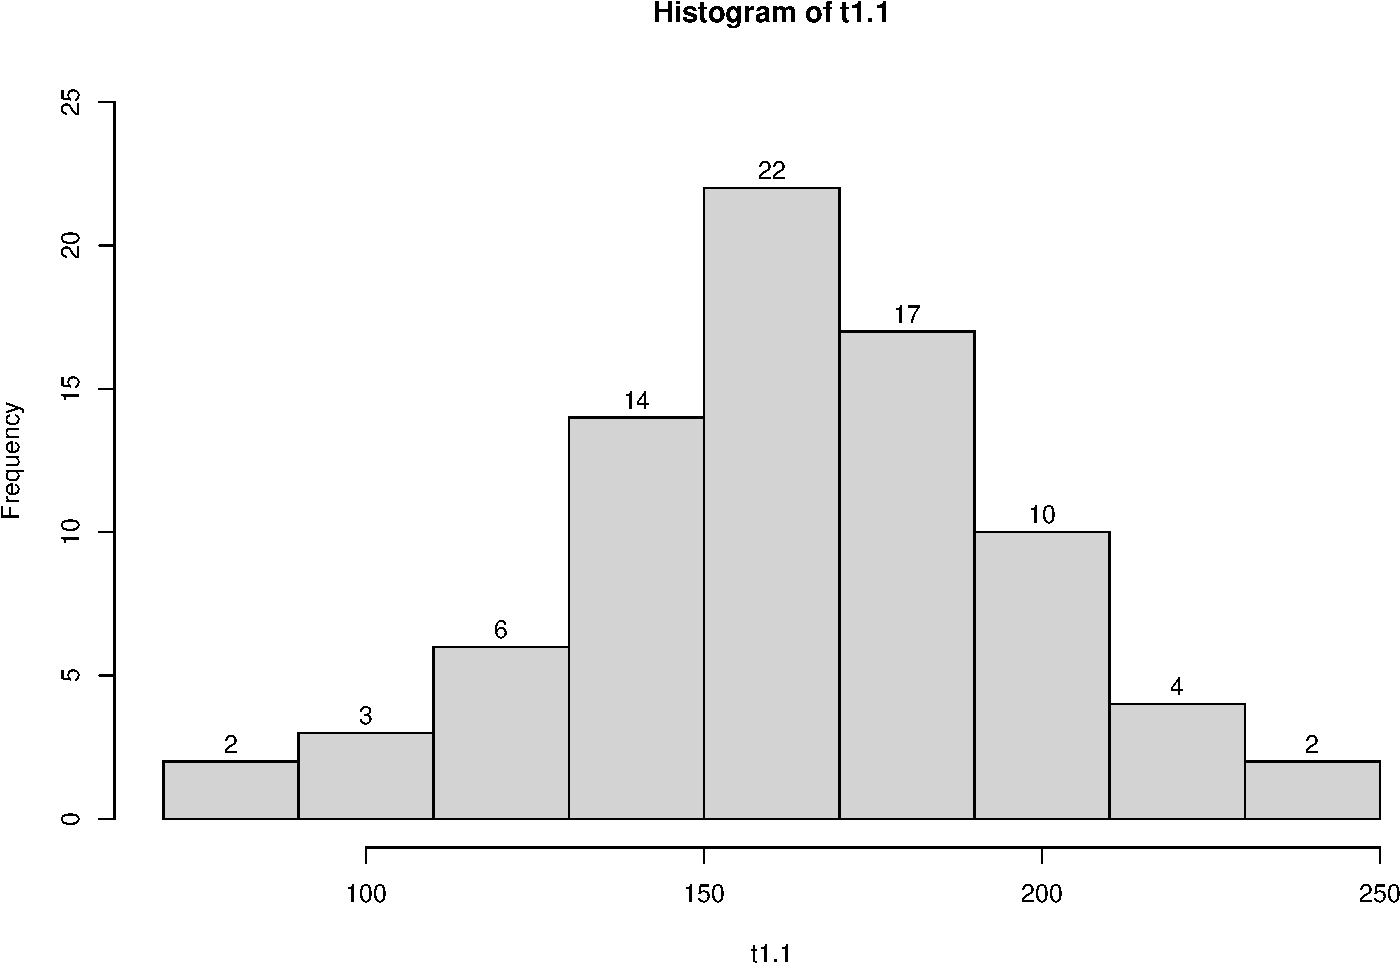
\includegraphics[keepaspectratio]{Listas_files/figure-beamer/unnamed-chunk-23-1.pdf}}
\end{frame}

\begin{frame}[fragile]{Solución}
\phantomsection\label{soluciuxf3n}
\begin{Shaded}
\begin{Highlighting}[]
\NormalTok{histo}\OtherTok{=}\FunctionTok{hist}\NormalTok{(t1}\FloatTok{.1}\NormalTok{,}\AttributeTok{breaks=}\FunctionTok{seq}\NormalTok{(}\DecValTok{70}\NormalTok{,}\DecValTok{250}\NormalTok{,}\AttributeTok{by=}\DecValTok{20}\NormalTok{),}\AttributeTok{right =} \ConstantTok{FALSE}\NormalTok{,}\AttributeTok{labels=}\ConstantTok{TRUE}\NormalTok{,}\AttributeTok{ylim=}\FunctionTok{c}\NormalTok{(}\DecValTok{0}\NormalTok{,}\DecValTok{25}\NormalTok{),}\AttributeTok{plot=}\ConstantTok{FALSE}\NormalTok{)   }
\end{Highlighting}
\end{Shaded}

Es \texttt{histo} una lista ?

\begin{Shaded}
\begin{Highlighting}[]
\FunctionTok{mode}\NormalTok{(histo)}
\end{Highlighting}
\end{Shaded}

\begin{verbatim}
[1] "list"
\end{verbatim}

\begin{Shaded}
\begin{Highlighting}[]
\FunctionTok{is.list}\NormalTok{(histo) }
\end{Highlighting}
\end{Shaded}

\begin{verbatim}
[1] TRUE
\end{verbatim}
\end{frame}

\begin{frame}[fragile]{Contenido de la lista}
\phantomsection\label{contenido-de-la-lista}
Qué cosas tengo dentro de esa lista?

\begin{Shaded}
\begin{Highlighting}[]
\FunctionTok{names}\NormalTok{(histo)}
\end{Highlighting}
\end{Shaded}

\begin{verbatim}
[1] "breaks"   "counts"   "density"  "mids"     "xname"    "equidist"
\end{verbatim}
\end{frame}

\begin{frame}[fragile]{Los límites de los intervalos}
\phantomsection\label{los-luxedmites-de-los-intervalos}
\begin{Shaded}
\begin{Highlighting}[]
\NormalTok{histo}\SpecialCharTok{$}\NormalTok{breaks}
\end{Highlighting}
\end{Shaded}

\begin{verbatim}
 [1]  70  90 110 130 150 170 190 210 230 250
\end{verbatim}

\begin{Shaded}
\begin{Highlighting}[]
\NormalTok{Li}\OtherTok{=}\NormalTok{histo}\SpecialCharTok{$}\NormalTok{breaks[}\SpecialCharTok{{-}}\FunctionTok{length}\NormalTok{(histo}\SpecialCharTok{$}\NormalTok{breaks)] }
\NormalTok{Li}
\end{Highlighting}
\end{Shaded}

\begin{verbatim}
[1]  70  90 110 130 150 170 190 210 230
\end{verbatim}

\begin{Shaded}
\begin{Highlighting}[]
\NormalTok{Ls}\OtherTok{=}\NormalTok{histo}\SpecialCharTok{$}\NormalTok{breaks[}\SpecialCharTok{{-}}\DecValTok{1}\NormalTok{] }
\NormalTok{Ls}
\end{Highlighting}
\end{Shaded}

\begin{verbatim}
[1]  90 110 130 150 170 190 210 230 250
\end{verbatim}
\end{frame}

\begin{frame}[fragile]{Limites de los intervalos}
\phantomsection\label{limites-de-los-intervalos}
\begin{Shaded}
\begin{Highlighting}[]
\FunctionTok{cbind}\NormalTok{(Li,Ls)}
\end{Highlighting}
\end{Shaded}

\begin{verbatim}
       Li  Ls
 [1,]  70  90
 [2,]  90 110
 [3,] 110 130
 [4,] 130 150
 [5,] 150 170
 [6,] 170 190
 [7,] 190 210
 [8,] 210 230
 [9,] 230 250
\end{verbatim}
\end{frame}

\begin{frame}[fragile]{Las marcas de clase}
\phantomsection\label{las-marcas-de-clase}
\begin{Shaded}
\begin{Highlighting}[]
\NormalTok{MC}\OtherTok{=}\NormalTok{histo}\SpecialCharTok{$}\NormalTok{mids}
\FunctionTok{cbind}\NormalTok{(Li,Ls,MC)}
\end{Highlighting}
\end{Shaded}

\begin{verbatim}
       Li  Ls  MC
 [1,]  70  90  80
 [2,]  90 110 100
 [3,] 110 130 120
 [4,] 130 150 140
 [5,] 150 170 160
 [6,] 170 190 180
 [7,] 190 210 200
 [8,] 210 230 220
 [9,] 230 250 240
\end{verbatim}
\end{frame}

\begin{frame}[fragile]{Las frecuencias absolutas y relativas}
\phantomsection\label{las-frecuencias-absolutas-y-relativas}
\begin{Shaded}
\begin{Highlighting}[]
\NormalTok{fi}\OtherTok{=}\NormalTok{histo}\SpecialCharTok{$}\NormalTok{counts}
\NormalTok{n}\OtherTok{=}\FunctionTok{sum}\NormalTok{(fi)}
\NormalTok{fir}\OtherTok{=}\NormalTok{fi}\SpecialCharTok{/}\NormalTok{n}
\FunctionTok{cbind}\NormalTok{(Li,Ls,MC,fi,fir)}
\end{Highlighting}
\end{Shaded}

\begin{verbatim}
       Li  Ls  MC fi    fir
 [1,]  70  90  80  2 0.0250
 [2,]  90 110 100  3 0.0375
 [3,] 110 130 120  6 0.0750
 [4,] 130 150 140 14 0.1750
 [5,] 150 170 160 22 0.2750
 [6,] 170 190 180 17 0.2125
 [7,] 190 210 200 10 0.1250
 [8,] 210 230 220  4 0.0500
 [9,] 230 250 240  2 0.0250
\end{verbatim}
\end{frame}

\begin{frame}[fragile]{Las frecuencias acumuladas y acumuladas
relativas}
\phantomsection\label{las-frecuencias-acumuladas-y-acumuladas-relativas}
\begin{Shaded}
\begin{Highlighting}[]
\NormalTok{Fi}\OtherTok{=}\FunctionTok{cumsum}\NormalTok{(fi)}
\NormalTok{Fir}\OtherTok{=}\NormalTok{Fi}\SpecialCharTok{/}\NormalTok{n}
\FunctionTok{cbind}\NormalTok{(Li,Ls,MC,fi,fir,Fi,Fir) }
\end{Highlighting}
\end{Shaded}

\begin{verbatim}
       Li  Ls  MC fi    fir Fi    Fir
 [1,]  70  90  80  2 0.0250  2 0.0250
 [2,]  90 110 100  3 0.0375  5 0.0625
 [3,] 110 130 120  6 0.0750 11 0.1375
 [4,] 130 150 140 14 0.1750 25 0.3125
 [5,] 150 170 160 22 0.2750 47 0.5875
 [6,] 170 190 180 17 0.2125 64 0.8000
 [7,] 190 210 200 10 0.1250 74 0.9250
 [8,] 210 230 220  4 0.0500 78 0.9750
 [9,] 230 250 240  2 0.0250 80 1.0000
\end{verbatim}
\end{frame}

\begin{frame}{La tabla en formato latex}
\phantomsection\label{la-tabla-en-formato-latex}
\begin{longtable}[]{@{}rrrrrrr@{}}
\toprule\noalign{}
Li & Ls & MC & fi & fir & Fi & Fir \\
\midrule\noalign{}
\endhead
70 & 90 & 80 & 2 & 0.0250 & 2 & 0.0250 \\
90 & 110 & 100 & 3 & 0.0375 & 5 & 0.0625 \\
110 & 130 & 120 & 6 & 0.0750 & 11 & 0.1375 \\
130 & 150 & 140 & 14 & 0.1750 & 25 & 0.3125 \\
150 & 170 & 160 & 22 & 0.2750 & 47 & 0.5875 \\
170 & 190 & 180 & 17 & 0.2125 & 64 & 0.8000 \\
190 & 210 & 200 & 10 & 0.1250 & 74 & 0.9250 \\
210 & 230 & 220 & 4 & 0.0500 & 78 & 0.9750 \\
230 & 250 & 240 & 2 & 0.0250 & 80 & 1.0000 \\
\bottomrule\noalign{}
\end{longtable}
\end{frame}

\begin{frame}{Aplicación}
\phantomsection\label{aplicaciuxf3n-1}
La media calculada a partir de datos agrupados en un histograma se
calcula con la siguiente formula
\[\bar{X}_a=\frac{\sum_{i=1}^k M_i\times f_i}{n}\] Donde \(M_i\) es la
marca de la clase \(i\), \(f_i\) es la frecuencia, \(n\) es el numero de
datos y \(k\) es el numero de intervalos. Recordemos que \(n=\sum f_i\).
\end{frame}

\begin{frame}[fragile]{Implementación}
\phantomsection\label{implementaciuxf3n}
A continuación se implementa la formula en R

\begin{Shaded}
\begin{Highlighting}[]
\FunctionTok{sum}\NormalTok{( histo}\SpecialCharTok{$}\NormalTok{counts}\SpecialCharTok{*}\NormalTok{histo}\SpecialCharTok{$}\NormalTok{mids )}\SpecialCharTok{/}\FunctionTok{sum}\NormalTok{(histo}\SpecialCharTok{$}\NormalTok{counts) }
\end{Highlighting}
\end{Shaded}

\begin{verbatim}
[1] 163.5
\end{verbatim}
\end{frame}

\begin{frame}{}
\phantomsection\label{section}
La media de los datos sin agrupar es 162.6625, se observa que no hay
mucha diferencia entre las dos medias, por lo tanto la media calculada a
partir de los datos agrupados en el histograma es una buena aproximación
de la media real de los datos.
\end{frame}

\begin{frame}{Ejercicio}
\phantomsection\label{ejercicio-2}
Calcular la varianza a partir de los datos agrupados y compararla con la
varianza de los datos sin agrupar.

Nota: La varianza con datos agrupados se obtiene con la siguiente
formula
\[S^2_a=\frac{\sum(M_i-\bar X_a)^2\times f_i }{n-1}=\frac{\sum M^2_if_i-n\bar X_a^2}{n-1}\]
\end{frame}

\section{Listas anidadas}\label{listas-anidadas}

\begin{frame}{Listas Anidadas}
\phantomsection\label{listas-anidadas-1}
\begin{itemize}
\item
  Dado que una lista puede contener \textbf{cualquier} tipo de objeto en
  R, ¡también puede albergar otras listas en su interior!
\item
  A esto se le conoce como una lista anidada.
\item
  Esta característica es muy poderosa porque nos permite crear
  estructuras jerárquicas complejas.
\end{itemize}
\end{frame}

\begin{frame}[fragile]{Ejemplo: lista anidada}
\phantomsection\label{ejemplo-lista-anidada}
\begin{Shaded}
\begin{Highlighting}[]
\CommentTok{\# Creamos una lista que contiene otra lista internamente}
\NormalTok{curso }\OtherTok{\textless{}{-}} \FunctionTok{list}\NormalTok{(}
  \AttributeTok{asignatura =} \StringTok{"Estadística Computacional"}\NormalTok{,}
  \AttributeTok{semestre =} \StringTok{"2026{-}2"}\NormalTok{,}
  \AttributeTok{notas =} \FunctionTok{list}\NormalTok{(}
    \AttributeTok{corte1 =} \FunctionTok{c}\NormalTok{(}\FloatTok{4.5}\NormalTok{, }\FloatTok{3.8}\NormalTok{, }\FloatTok{4.0}\NormalTok{),}
    \AttributeTok{corte2 =} \FunctionTok{c}\NormalTok{(}\FloatTok{3.2}\NormalTok{, }\FloatTok{4.1}\NormalTok{, }\FloatTok{4.8}\NormalTok{)}
\NormalTok{  )}
\NormalTok{)}
\end{Highlighting}
\end{Shaded}
\end{frame}

\begin{frame}[fragile]{Indexado en Listas Anidadas}
\phantomsection\label{indexado-en-listas-anidadas}
Para acceder a los elementos profundos (``sub-elementos'') de una lista
anidada, simplemente debemos encadenar los operadores de extracción, ya
sea el signo \texttt{\$} o los dobles corchetes \texttt{{[}{[}{]}{]}}.

\begin{Shaded}
\begin{Highlighting}[]
\CommentTok{\# Encadenando el signo $ (Muy intuitivo)}
\NormalTok{curso}\SpecialCharTok{$}\NormalTok{notas}\SpecialCharTok{$}\NormalTok{corte1}
\end{Highlighting}
\end{Shaded}

\begin{verbatim}
[1] 4.5 3.8 4.0
\end{verbatim}
\end{frame}

\begin{frame}[fragile]{Con dobles corchetes \texttt{{[}{[}{]}{]}}}
\phantomsection\label{con-dobles-corchetes}
\begin{Shaded}
\begin{Highlighting}[]
\CommentTok{\# Encadenando dobles corchetes (Elemento 3, sub{-}elemento 2)}
\NormalTok{curso[[}\DecValTok{3}\NormalTok{]][[}\DecValTok{2}\NormalTok{]]}
\end{Highlighting}
\end{Shaded}

\begin{verbatim}
[1] 3.2 4.1 4.8
\end{verbatim}
\end{frame}

\begin{frame}[fragile]{Ejercicio}
\phantomsection\label{ejercicio-3}
Calcular la nota promedio del segundo corte

\begin{Shaded}
\begin{Highlighting}[]
\CommentTok{\# Calculando la media de un sub{-}elemento}
\FunctionTok{mean}\NormalTok{(curso}\SpecialCharTok{$}\NormalTok{notas}\SpecialCharTok{$}\NormalTok{corte2)}
\end{Highlighting}
\end{Shaded}

\begin{verbatim}
[1] 4.033333
\end{verbatim}
\end{frame}

\section{Iteración en listas}\label{iteraciuxf3n-en-listas}

\begin{frame}[fragile]{Iteración en Listas: Familia \texttt{apply}}
\phantomsection\label{iteraciuxf3n-en-listas-familia-apply}
En R, es muy común querer realizar la \textbf{misma operación matemática
o estadística} sobre cada uno de los elementos de una lista.

Aunque esto se puede hacer con un bucle \texttt{for}, en R la mejor
práctica (y la más rápida) es usar la familia de funciones
\texttt{apply}. Hoy nos enfocaremos en dos de las más importantes para
listas:

\begin{itemize}
\tightlist
\item
  \texttt{lapply()}: Devuelve siempre una \textbf{l}ista.
\item
  \texttt{sapply()}: Devuelve un resultado \textbf{s}implificado
  (usualmente un vector).
\end{itemize}
\end{frame}

\begin{frame}[fragile]{La función \texttt{lapply()}}
\phantomsection\label{la-funciuxf3n-lapply}
La función \texttt{lapply()} (List Apply) toma una lista, aplica una
función a cada uno de sus elementos y \textbf{siempre devuelve otra
lista} de la misma longitud.

\begin{Shaded}
\begin{Highlighting}[]
\CommentTok{\# Creamos una lista con tres vectores numéricos}
\NormalTok{notas\_estudiantes }\OtherTok{\textless{}{-}} \FunctionTok{list}\NormalTok{(}
  \AttributeTok{Juan =} \FunctionTok{c}\NormalTok{(}\FloatTok{4.0}\NormalTok{, }\FloatTok{3.5}\NormalTok{, }\FloatTok{4.2}\NormalTok{),}
  \AttributeTok{Maria =} \FunctionTok{c}\NormalTok{(}\FloatTok{4.8}\NormalTok{, }\FloatTok{5.0}\NormalTok{, }\FloatTok{4.6}\NormalTok{),}
  \AttributeTok{Pedro =} \FunctionTok{c}\NormalTok{(}\FloatTok{3.1}\NormalTok{, }\FloatTok{2.8}\NormalTok{, }\FloatTok{3.5}\NormalTok{)}
\NormalTok{)}

\CommentTok{\# Calculamos la media de cada estudiante}
\NormalTok{medias\_lista }\OtherTok{\textless{}{-}} \FunctionTok{lapply}\NormalTok{(notas\_estudiantes, mean)}
\NormalTok{medias\_lista}
\end{Highlighting}
\end{Shaded}

\begin{verbatim}
$Juan
[1] 3.9

$Maria
[1] 4.8

$Pedro
[1] 3.133333
\end{verbatim}
\end{frame}

\begin{frame}[fragile]{La función \texttt{sapply()}}
\phantomsection\label{la-funciuxf3n-sapply}
\begin{itemize}
\item
  La función \texttt{sapply()} (Simplified Apply) hace exactamente el
  mismo cálculo que \texttt{lapply()}, pero intenta simplificar el
  resultado final.
\item
  Si el resultado de la función es un solo número por cada elemento
  (como la media), \texttt{sapply()} lo agrupa todo elegantemente en un
  vector numérico.
\end{itemize}
\end{frame}

\begin{frame}[fragile]{Uso de \texttt{sapply()}}
\phantomsection\label{uso-de-sapply}
\begin{Shaded}
\begin{Highlighting}[]
\CommentTok{\# Mismo cálculo, pero con sapply}
\NormalTok{medias\_vector }\OtherTok{\textless{}{-}} \FunctionTok{sapply}\NormalTok{(notas\_estudiantes, mean)}
\NormalTok{medias\_vector}
\end{Highlighting}
\end{Shaded}

\begin{verbatim}
    Juan    Maria    Pedro 
3.900000 4.800000 3.133333 
\end{verbatim}
\end{frame}

\begin{frame}[fragile]{Argumentos adicionales en \texttt{apply}}
\phantomsection\label{argumentos-adicionales-en-apply}
\begin{itemize}
\item
  Tanto \texttt{lapply()} como \texttt{sapply()} permiten pasarle
  argumentos adicionales a la función que estamos aplicando.
\item
  Por ejemplo, si uno de los estudiantes faltó a un examen y tiene un
  NA:
\end{itemize}

\begin{Shaded}
\begin{Highlighting}[]
\NormalTok{notas\_con\_na }\OtherTok{\textless{}{-}} \FunctionTok{list}\NormalTok{(}\AttributeTok{Juan =} \FunctionTok{c}\NormalTok{(}\FloatTok{4.0}\NormalTok{, }\FloatTok{3.5}\NormalTok{, }\FloatTok{4.2}\NormalTok{), }\AttributeTok{Ana =} \FunctionTok{c}\NormalTok{(}\FloatTok{4.5}\NormalTok{, }\ConstantTok{NA}\NormalTok{, }\FloatTok{4.0}\NormalTok{))}

\CommentTok{\# Agregamos na.rm = TRUE como tercer argumento}
\FunctionTok{sapply}\NormalTok{(notas\_con\_na, mean, }\AttributeTok{na.rm =} \ConstantTok{TRUE}\NormalTok{)}
\end{Highlighting}
\end{Shaded}

\begin{verbatim}
Juan  Ana 
3.90 4.25 
\end{verbatim}
\end{frame}




\end{document}
